\documentclass{beamer}

\mode<presentation>
{
  \usetheme{Warsaw}
  \setbeamercovered{transparent}
}

\usepackage[english]{babel}
\usepackage[utf8]{inputenc}
\usepackage{times}
\usepackage[T1]{fontenc}
\usepackage{graphicx}
\graphicspath{ {images/} }

\title[]
{DŁUG TECHNICZNY\\
Narzędzie profesjonalisty}

\author[Adrian Mularczyk]{Adrian Mularczyk}

\institute[PGS Softwarei]
{
PGS Software
}

\date{}

\begin{document}

\begin{frame}
  \titlepage 
\end{frame}

\begin{frame}{}
\Huge{Krzysztof Kędzierski\newline\newline}
\Large{"Dług techniczny - Narzędzie Profesjonalisty"\newline\newline}
\Large{konferencja Boiling Frogs 2018\newline\newline\newline}
\Large{https://www.youtube.com/watch?v=PxcQlSUIpjQ}
\end{frame}

\begin{frame}{Agenda}
  \tableofcontents
\end{frame}

\section{Wyjaśnienie problemu}

\begin{frame}{}
\begin{center}
\Huge{Wyjaśnienie problemu}
\end{center}
\end{frame}

\begin{frame}{}
\begin{center}
\Large{Nasz kod + nowe wymagania = dług techniczny}
\end{center}
\end{frame}


\section{Dług techniczny}

\begin{frame}{Dług techniczny}
\begin{center}
\Huge{Dług techniczny}
\end{center}
\end{frame}

\begin{frame}{Tetris}
\begin{center}
  	
\includegraphics[height=6cm]{tetris.jpg}
\end{center}
\end{frame}

\begin{frame}{\textit{Design Stamina Hipotesis}}
\begin{center}
  	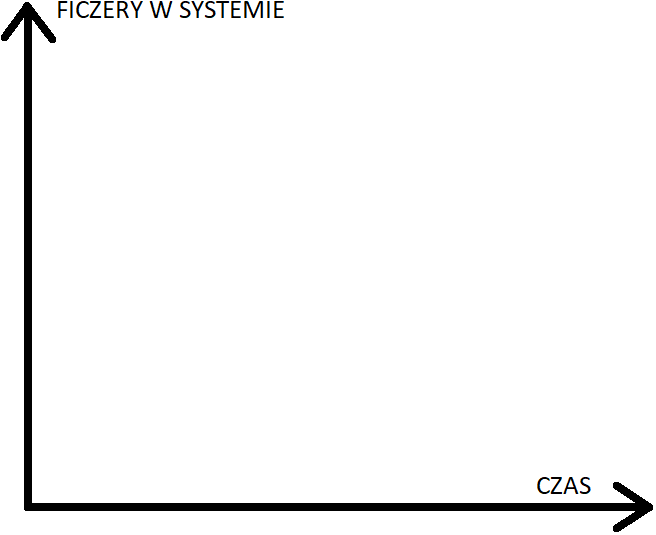
\includegraphics[height=6cm]{design_stability_hipotesis1.png}
\end{center}
\end{frame}

\begin{frame}{\textit{Design Stamina Hipotesis}}
\begin{center}
  	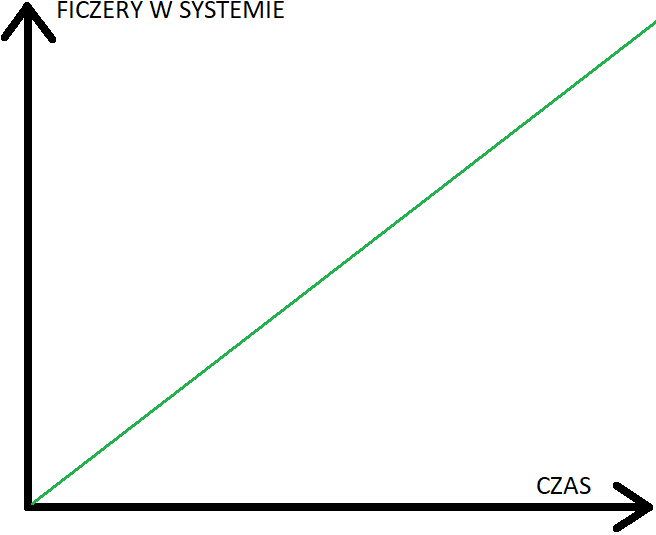
\includegraphics[height=6cm]{design_stability_hipotesis2.png}
\end{center}
\end{frame}

\begin{frame}{\textit{Design Stamina Hipotesis}}
\begin{center}
  	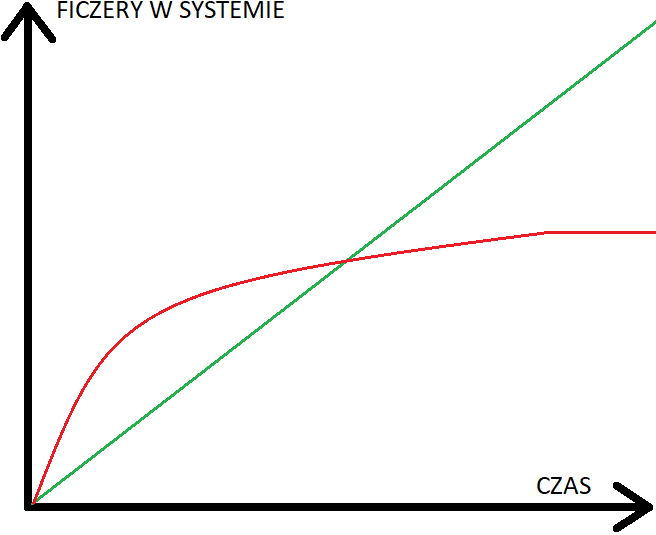
\includegraphics[height=6cm]{design_stability_hipotesis3.png}
\end{center}
\end{frame}

\begin{frame}{\textit{Design Stamina Hipotesis}}
\begin{center}
  	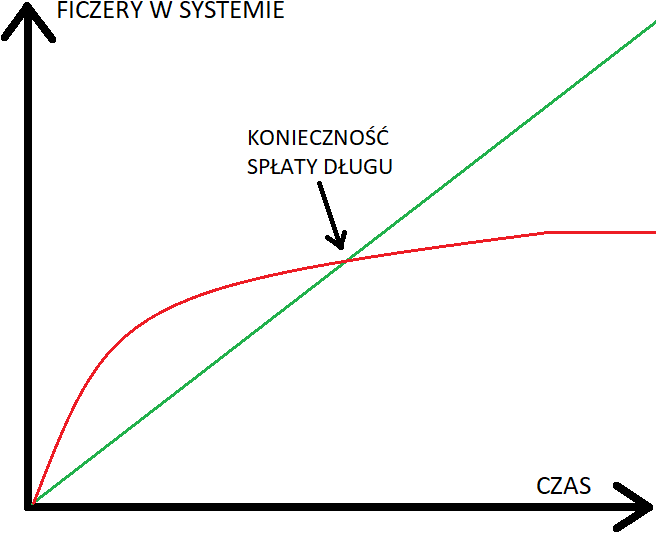
\includegraphics[height=6cm]{design_stability_hipotesis4.png}
\end{center}
\end{frame}

\section{Spłacalny dług techniczny}

\begin{frame}{}
\begin{center}
\Huge{Spłacalny dług techniczny}
\end{center}
\end{frame}

\begin{frame}{}
\begin{center}
\Huge{\textit{Technical debt quadrant}}
\end{center}
\end{frame}

\begin{frame}{\textit{Technical debt quadrant}}
\begin{center}
  	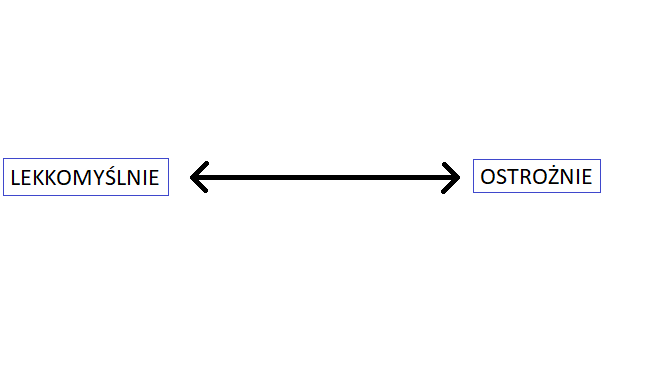
\includegraphics[height=6cm]{technical_debt_quadrant1.png}
\end{center}
\end{frame}

\begin{frame}{\textit{Technical debt quadrant}}
\begin{center}
  	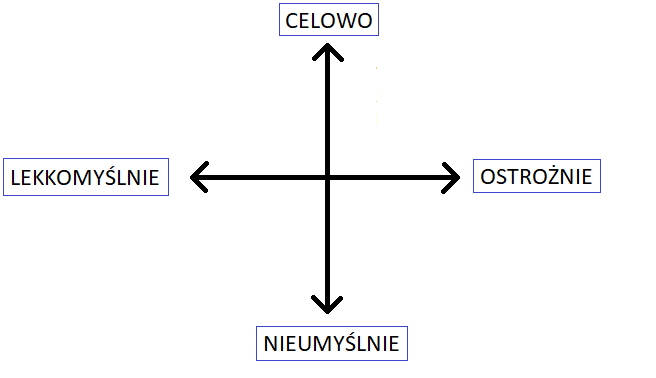
\includegraphics[height=6cm]{technical_debt_quadrant2.png}
\end{center}
\end{frame}

\begin{frame}{\textit{Technical debt quadrant}}
\begin{center}
  	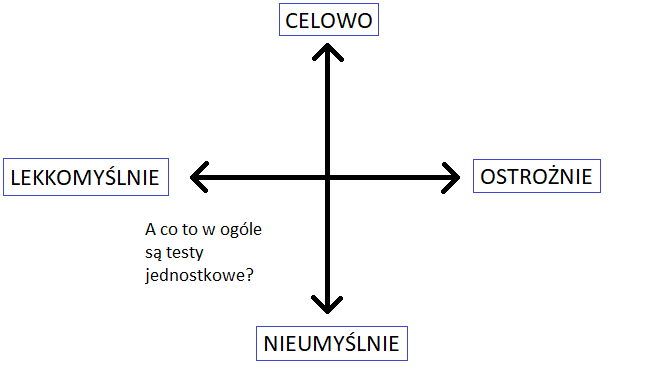
\includegraphics[height=6cm]{technical_debt_quadrant3.png}
\end{center}
\end{frame}

\begin{frame}{\textit{Technical debt quadrant}}
\begin{center}
  	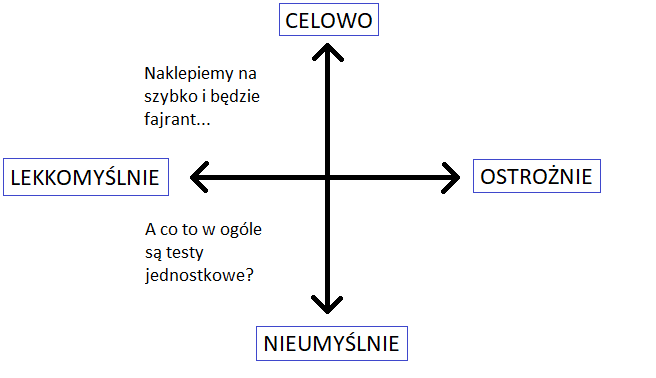
\includegraphics[height=6cm]{technical_debt_quadrant4.png}
\end{center}
\end{frame}

\begin{frame}{\textit{Technical debt quadrant}}
\begin{center}
  	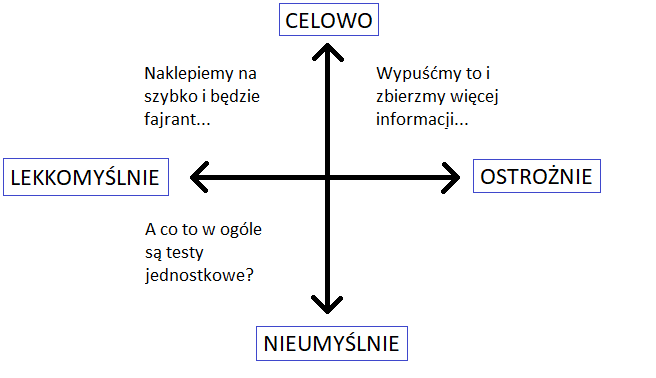
\includegraphics[height=6cm]{technical_debt_quadrant5.png}
\end{center}
\end{frame}

\begin{frame}{\textit{Technical debt quadrant}}
\begin{center}
  	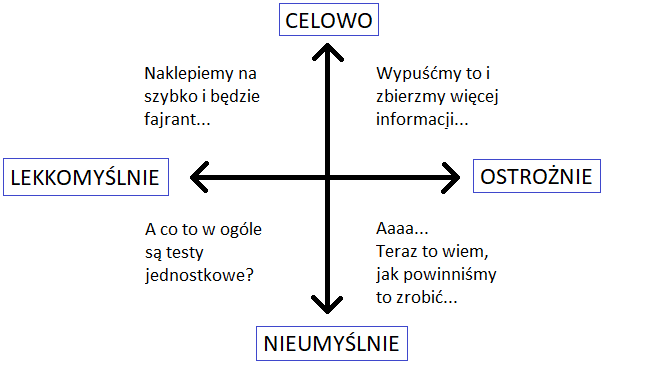
\includegraphics[height=6cm]{technical_debt_quadrant6.png}
\end{center}
\end{frame}

\begin{frame}{Czy możliwa jest spłata długu{?}}
\begin{center}
  	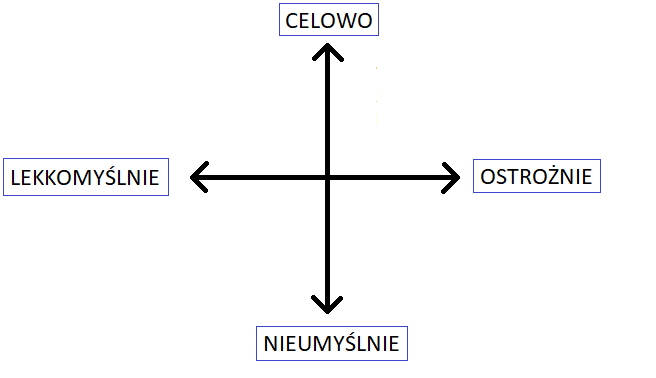
\includegraphics[height=6cm]{splata_dlugu1.png}
\end{center}
\end{frame}

\begin{frame}{Czy możliwa jest spłata długu{?}}
\begin{center}
  	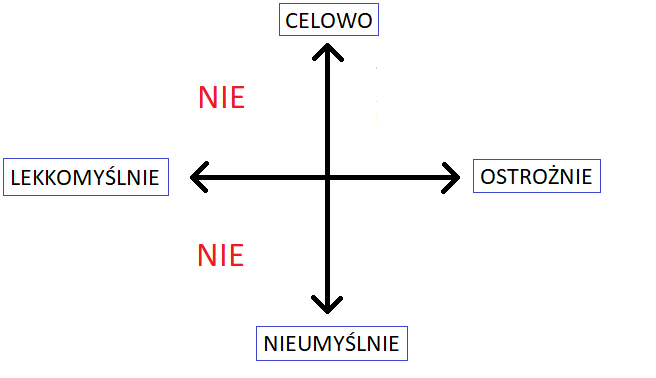
\includegraphics[height=6cm]{splata_dlugu2.png}
\end{center}
\end{frame}

\begin{frame}{Czy możliwa jest spłata długu{?}}
\begin{center}
  	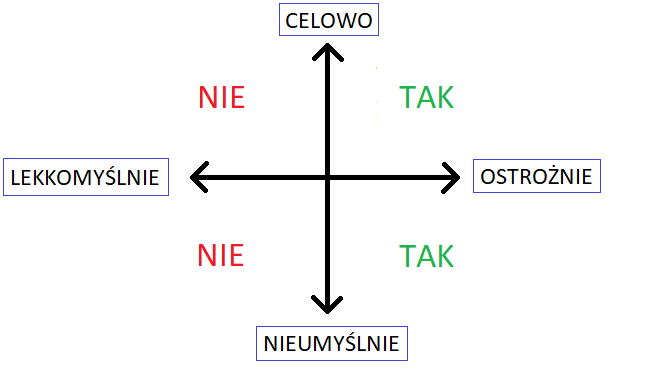
\includegraphics[height=6cm]{splata_dlugu3.png}
\end{center}
\end{frame}

\begin{frame}{Spłacalny dług techniczny}
     \begin{Large}
	\begin{itemize}
		\item Piszmy czysty kod
		\item 
		\item 
		\item 
		\item 
	\end{itemize}
     \end{Large}
\end{frame}

\begin{frame}{}
\begin{center}
  	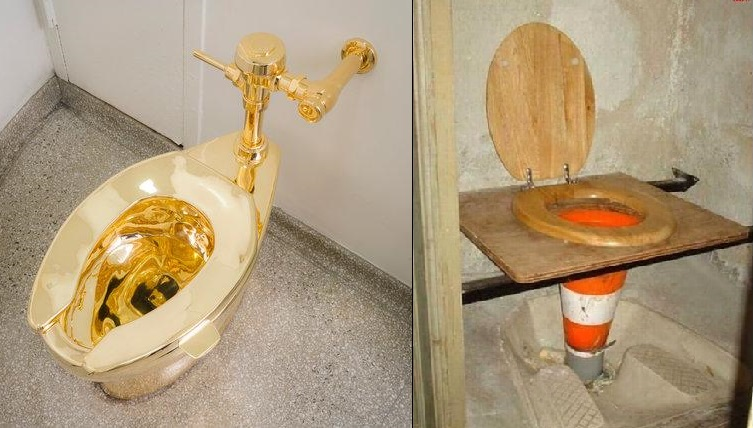
\includegraphics[height=6cm]{prosty_kod1.jpg}
\end{center}
\end{frame}

\begin{frame}{}
\begin{center}
  	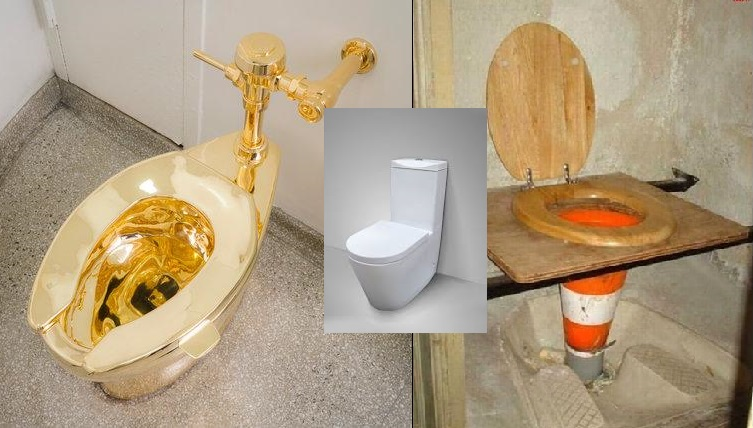
\includegraphics[height=6cm]{prosty_kod2.jpg}
\end{center}
\end{frame}

\begin{frame}{}
     \begin{Large}
	\begin{itemize}
		\item Piszmy czysty kod
		\item Piszmy prosty kod
		\item 
		\item 
		\item 
	\end{itemize}
     \end{Large}
\end{frame}

\begin{frame}{Zasada Pareto}
\begin{center}
  	
\includegraphics[height=6cm]{pareto.jpg}
\end{center}
\end{frame}

\begin{frame}{Zasada Pareto}
\begin{center}
\Large{{\color{red}X\%} KODU ODPOWIADA\\
ZA {\color{red}Y\%} ZŁOŻONOŚCI/PROBLEMÓW}
\end{center}
\end{frame}

\begin{frame}{Zasada Pareto}
\begin{center}
\Large{{\color{red}5\%} KODU ODPOWIADA\\
ZA {\color{red}95\%} ZŁOŻONOŚCI/PROBLEMÓW}
\end{center}
\end{frame}

\begin{frame}{git log --pretty=format:'\%ad \%aN \%s' --numstat}
\begin{center}
  	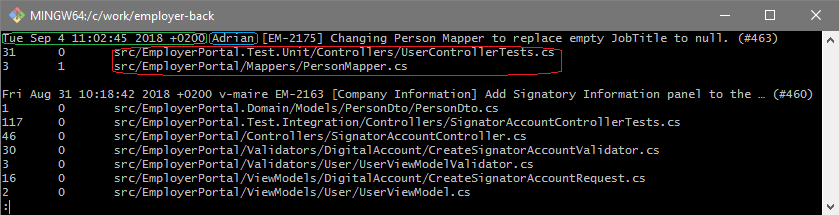
\includegraphics[height=4.85cm]{git_log.png}
\end{center}
\end{frame}

\begin{frame}{}
\begin{center}
  	
\includegraphics[height=6cm]{git_log1.png}
\end{center}
\end{frame}

\begin{frame}{}
\begin{center}
  	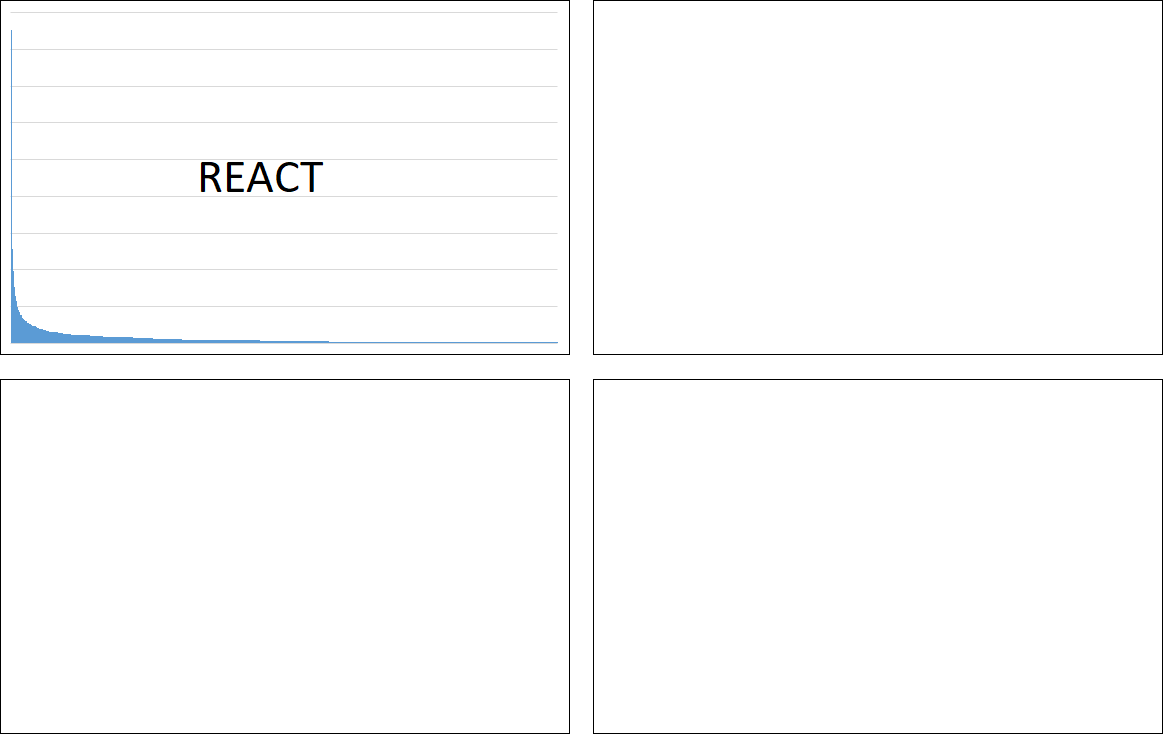
\includegraphics[height=6cm]{git_log2.png}
\end{center}
\end{frame}

\begin{frame}{}
\begin{center}
  	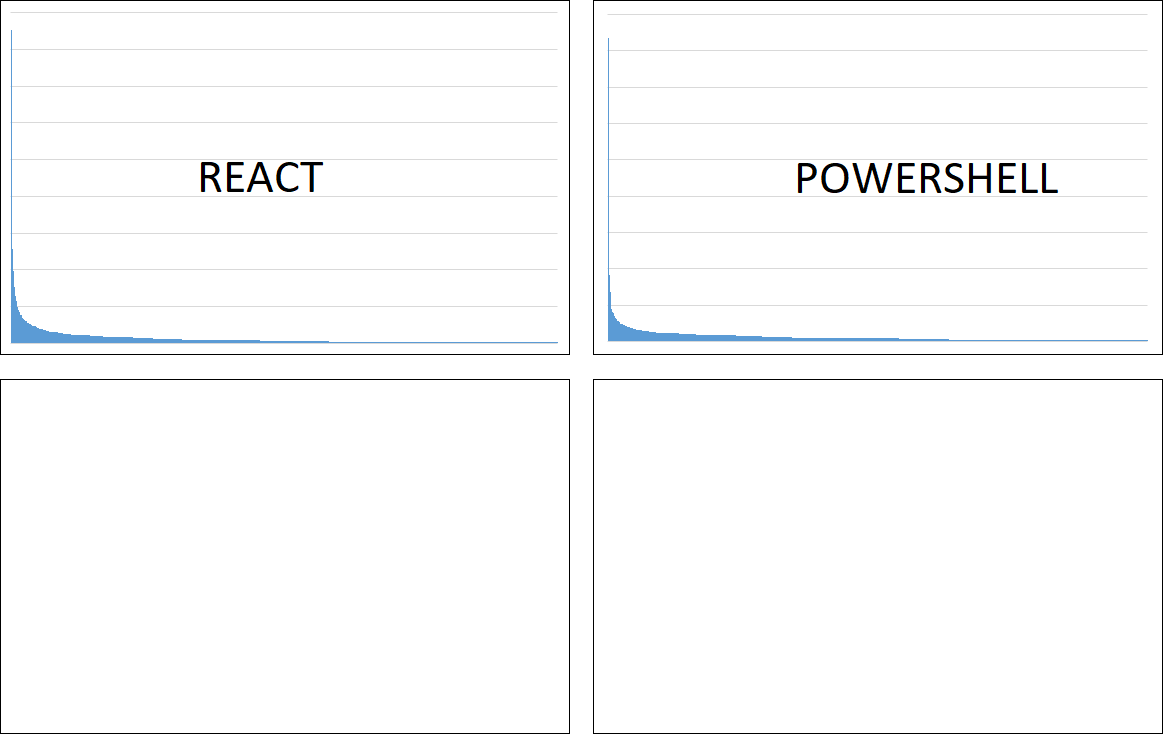
\includegraphics[height=6cm]{git_log3.png}
\end{center}
\end{frame}

\begin{frame}{}
\begin{center}
  	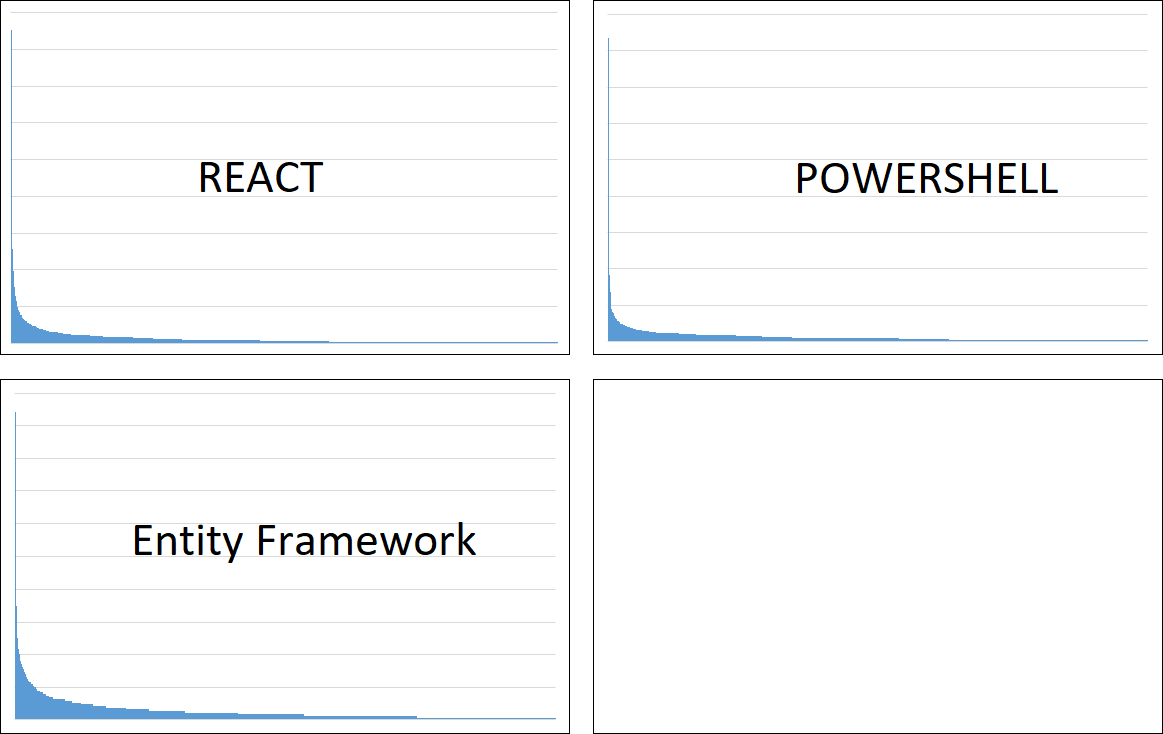
\includegraphics[height=6cm]{git_log4.png}
\end{center}
\end{frame}

\begin{frame}{}
\begin{center}
  	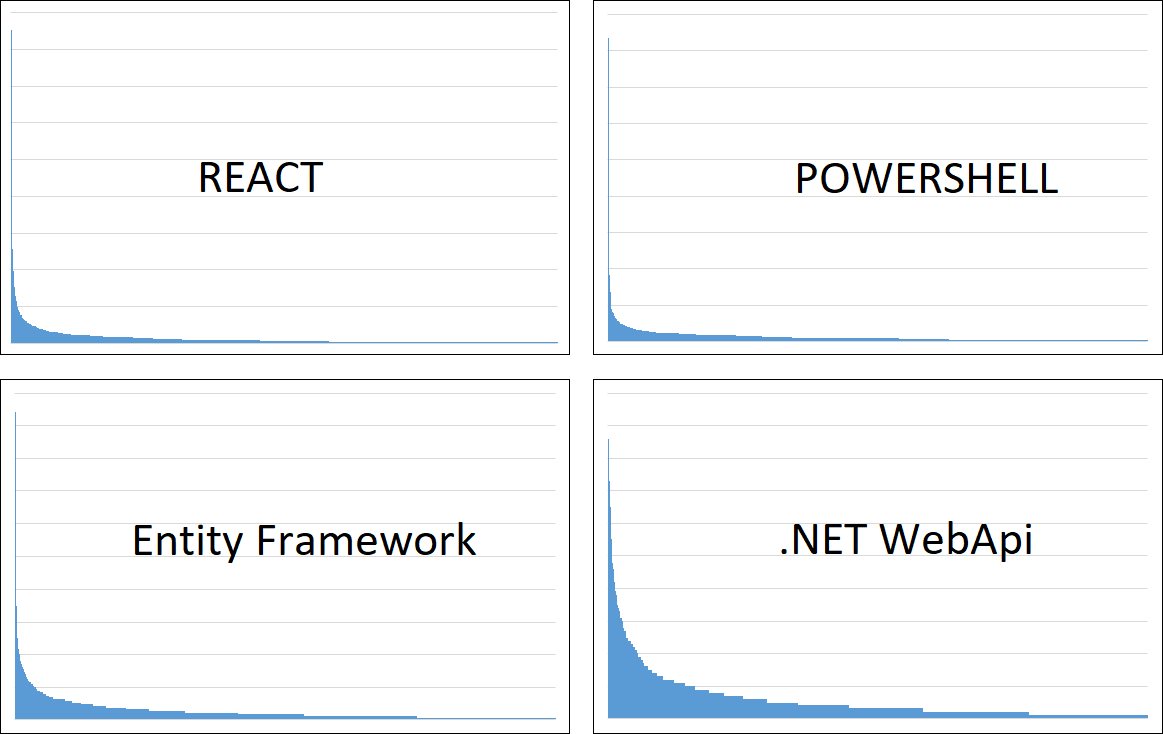
\includegraphics[height=6cm]{git_log5.png}
\end{center}
\end{frame}

\begin{frame}{}
\begin{center}
  	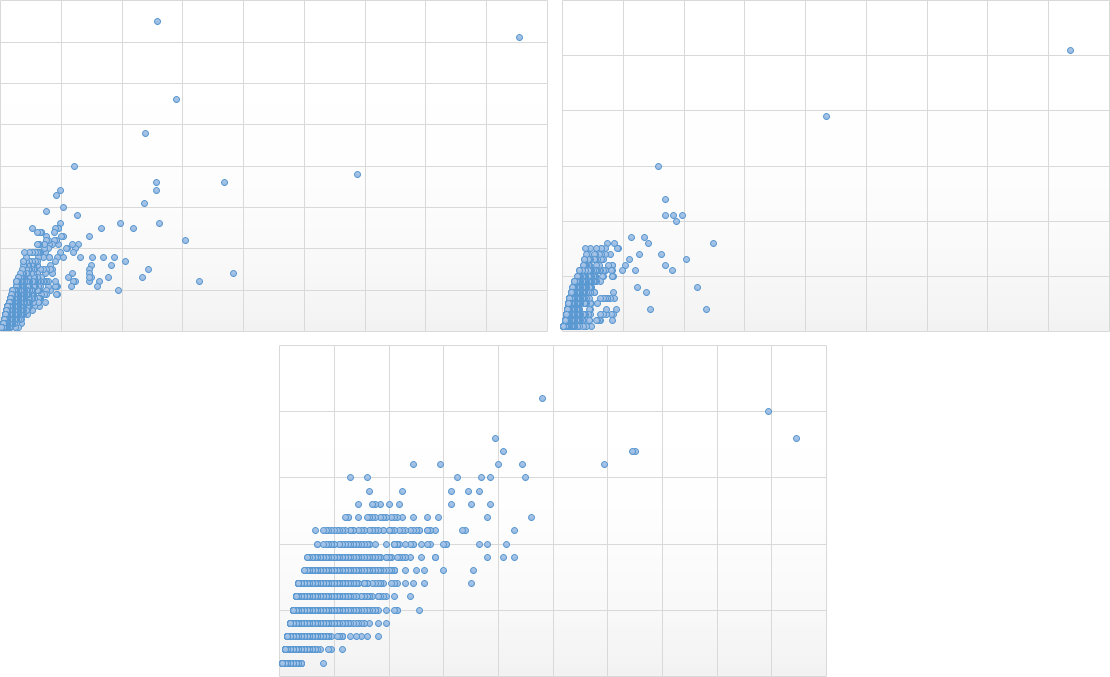
\includegraphics[height=6cm]{git_advanced.png}
\end{center}
\end{frame}

\begin{frame}{}
     \begin{Large}
	\begin{itemize}
		\item Piszmy czysty kod
		\item Piszmy prosty kod
		\item Monitorujmy gdzie narastają odsetki
		\item 
		\item 
	\end{itemize}
     \end{Large}
\end{frame}

\begin{frame}{}
\begin{center}
  	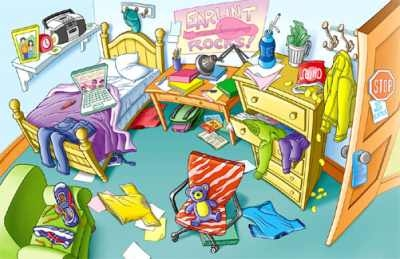
\includegraphics[height=6cm]{mess.jpeg}
\end{center}
\end{frame}

\begin{frame}{}
\begin{center}
\Huge{PGF}
\end{center}
\end{frame}

\begin{frame}{}
\begin{center}
  	
\includegraphics[height=6cm]{pgf1.jpg}
\end{center}
\end{frame}

\begin{frame}{}
\begin{center}
  	
\includegraphics[height=6cm]{pgf2.jpg}
\end{center}
\end{frame}

\begin{frame}{}
\begin{center}
  	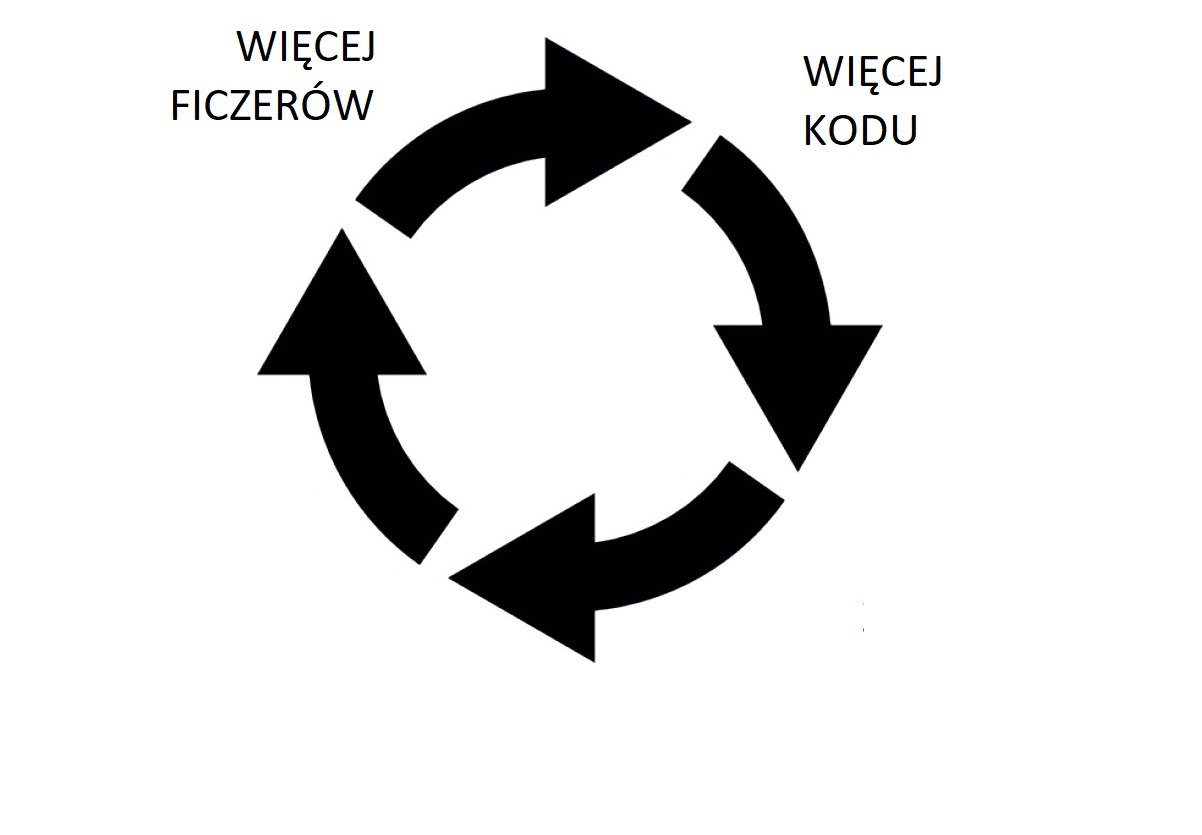
\includegraphics[height=6cm]{pgf3.jpg}
\end{center}
\end{frame}

\begin{frame}{}
\begin{center}
  	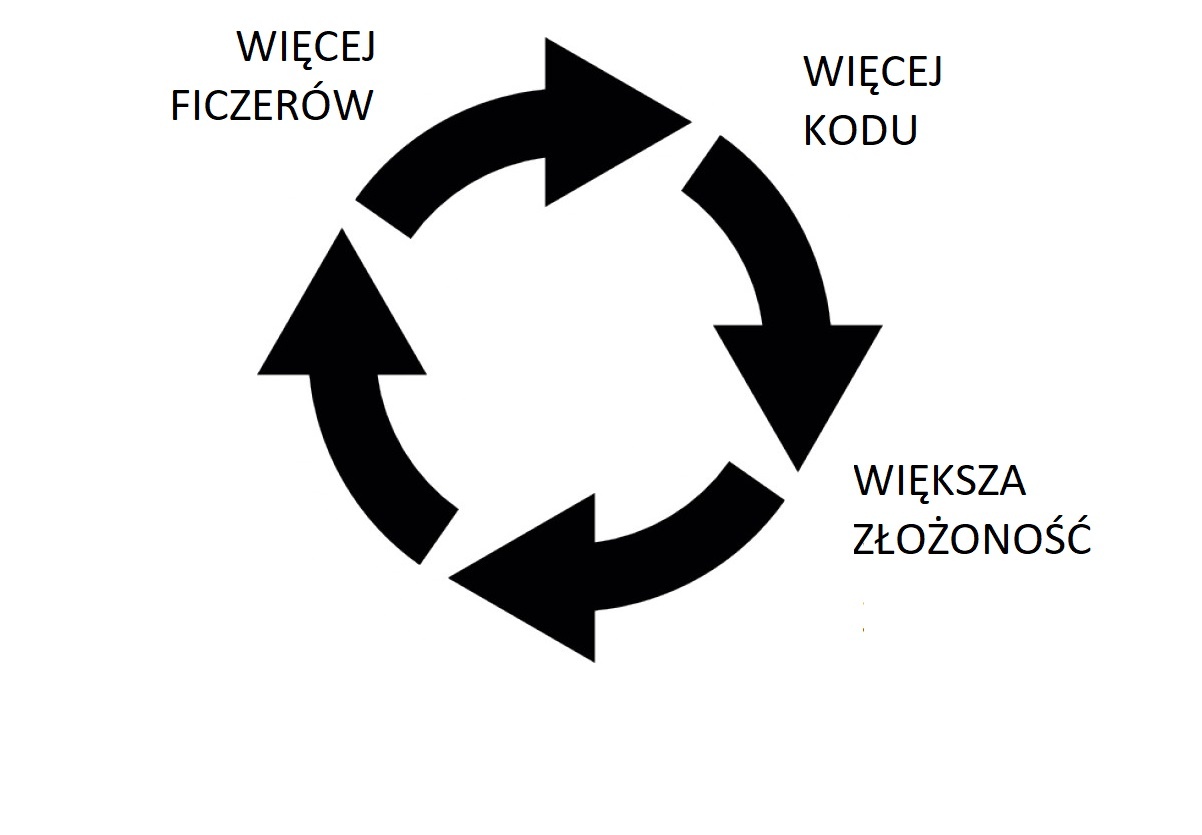
\includegraphics[height=6cm]{pgf4.jpg}
\end{center}
\end{frame}

\begin{frame}{}
\begin{center}
  	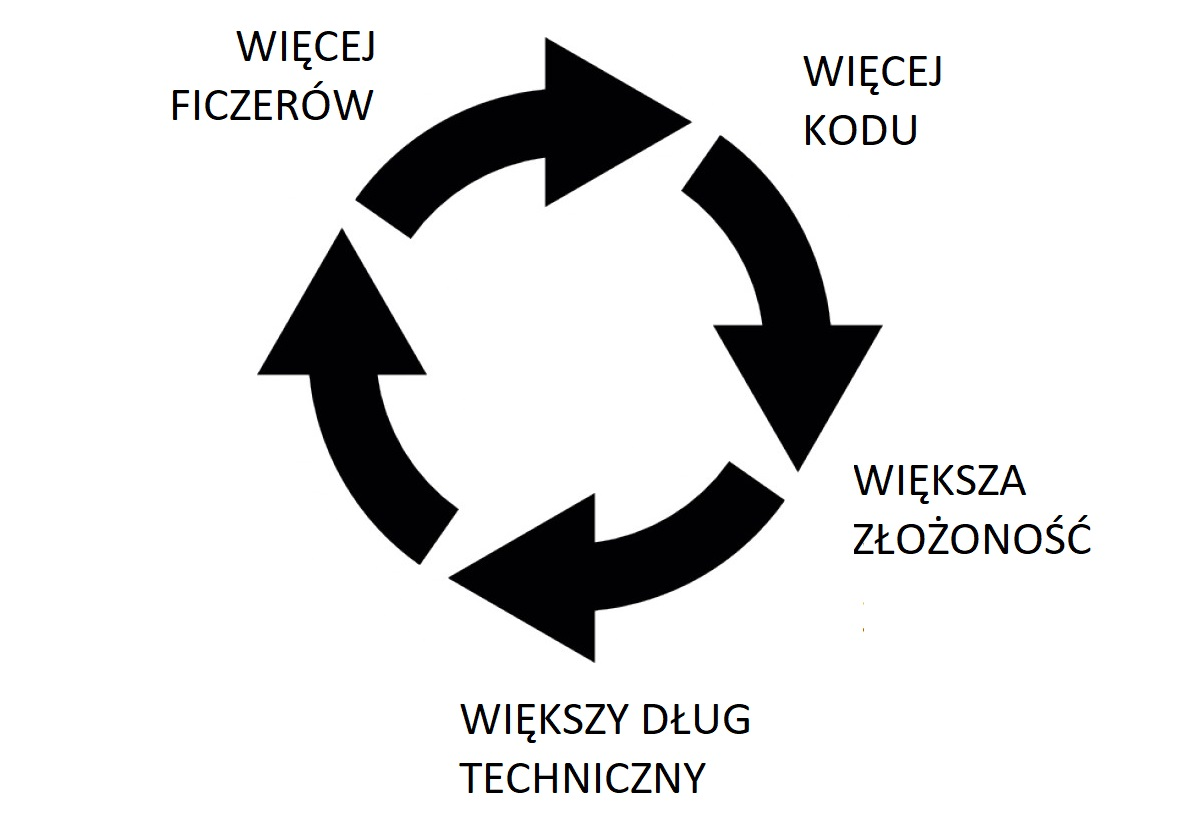
\includegraphics[height=6cm]{pgf5.jpg}
\end{center}
\end{frame}

\begin{frame}{}
\begin{center}
  	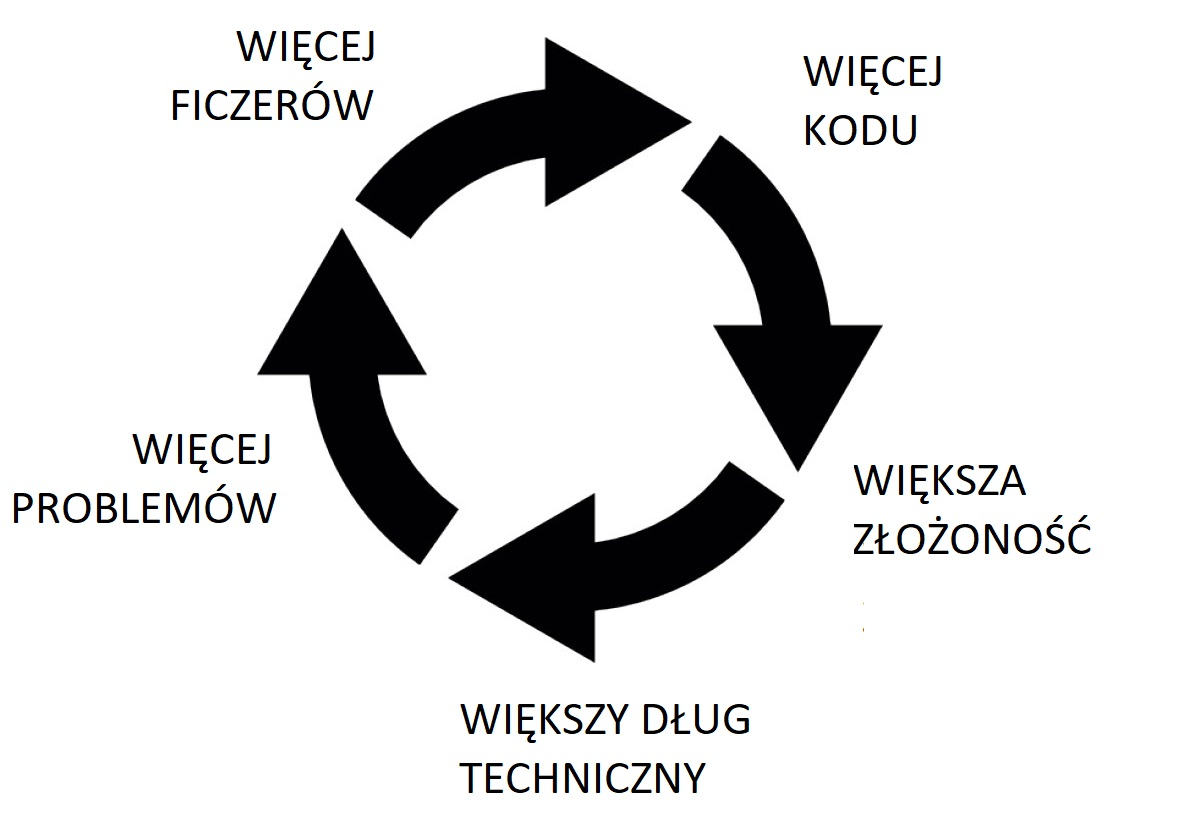
\includegraphics[height=6cm]{pgf6.jpg}
\end{center}
\end{frame}

\begin{frame}{}
\begin{center}
  	
\includegraphics[height=6cm]{pgf7.jpg}
\end{center}
\end{frame}

\begin{frame}{Pętla gnijących ficzerów}
\begin{center}
  	
\includegraphics[height=6cm]{pgf7.jpg}
\end{center}
\end{frame}

\begin{frame}{}
     \begin{Large}
	\begin{itemize}
		\item Piszmy czysty kod
		\item Piszmy prosty kod
		\item Monitorujmy gdzie narastają odsetki
		\item Usuwajmy nieużywane funkcjonalności
		\item 
	\end{itemize}
     \end{Large}
\end{frame}


\begin{frame}{Co jest problemem?}
\begin{center}
  	
\includegraphics[height=6cm]{problem.jpg}
\end{center}
\end{frame}

\begin{frame}{}
\begin{center}
\Huge{Wymagania}
\end{center}
\end{frame}

\begin{frame}{}
\begin{center}
  	
\includegraphics[height=6cm]{agile.png}
\end{center}
\end{frame}

\begin{frame}{}
\begin{center}
{\color{red}\Large{We cannot be agile if our code sucks...}}
\end{center}
\end{frame}

\begin{frame}{}
     \begin{Large}
	\begin{itemize}
		\item Piszmy czysty kod
		\item Piszmy prosty kod
		\item Monitorujmy gdzie narastają odsetki
		\item Usuwajmy nieużywane funkcjonalności
		\item Traktujmy siebie jako profesjonalistów
	\end{itemize}
     \end{Large}
\end{frame}


\begin{frame}{Pytania?}
\begin{center}
\Huge{Dziękuję!}\\
\Large{e-mail: amularczyk@pgs-soft.com}
\end{center}
\end{frame}


\end{document}